\chapter{Felhasználói dokumentáció}
\label{ch:user}

\section{Rendszerkövetelmények}

\subsection{Futtatás}

Magának webalkalmazás szerveroldalának a futtatásához a ASP.NET Core Runtime 8.0-ra van szükség, amelyhez
szükséges az alábbi operációs rendszerek valamelyike:
\begin{compactitem}
	\item Windows 10, 11 vagy Server 2012+
	\item 64-bites Ubuntu 20.04+ vagy Debian 11+
	\item macOS 10.15+ (csak külső, hosztolt szerver esetén támogatott)
\end{compactitem} 
A memóriahasználat a felhasználóktól nagyban függ, így 0,5 GB-tól akár 4 GB RAM-ra is szüksége lehet a szervernek a zökkenőmentes futáshoz. A merevlemezen történő tárhelyhasználat nagyban függ az éppen bejelentett pontok méretétől és legfőképp az azokhoz csatolt fényképektől. Magához a futtatáshoz elegendő 0,5 GB tárhely is (az ehhez szükséges szoftvereket nem bele értve), viszont az alkalmazás használtat közben ez nagy mértékben fog növekedni az előbb említett okok miatt, így érdemes akár saját, nagy kapacitású merevlemezre telepíteni a szerveroldalt.
Az szerver által használt SQL Server adatbázishoz (későbbiekben MSSQL-adatbázis) a Microsoft SQL Server szoftver valamelyik, de lehetőség szerint a legfrissebb, 2019-es verziójára van szükség, melyet a fentebb említett operációs rendszerek bármelyike képes futtatni.
Az első üzembe helyezést követően nincsen szükség további rendszergazdai feladatokra.
\subsection{Használat}

A program felhasználói felülete egy weboldal. Ennek meglátogatásához elsősorban szükség van egy olyan operációs rendszer telepítésére, majd futtatására, melyre elérhető bármilyen friss, Chromium-alapú webböngésző. Egy ilyen böngésző a Google Chrome, amellyel ajánlott a weboldal látogatása. Hardver- és szoftver követelményei az alábbiak:
\begin{compactitem}
	\item Operációs rendszerek valamelyike:
	\begin{compactitem}
		\item Windows 10, 11 vagy Server 2012+
		\item 64-bites Ubuntu 20.04+ vagy Debian 11+
		\item macOS 10.15+
		\item Android 8.0+ vagy Chrome OS
	\end{compactitem}
	\item Minimális hardver követelmények:
	\begin{compactitem}
		\item Pentium 4+ (vagy más, SSE3-at támogató) processzor
		\item 2 (ajánlottan 4) GB RAM
	\end{compactitem}
\end{compactitem}

Felhasználóként első üzembe helyezésre nincsen szükség, elég ha a felhasználó meglátogatja az oldalt. Ha még nem regisztrált felhasználói fiókot, akkor bizonyos funkciók eléréséhez regisztrálnia kell.

\section{Általános felhasználói tájékoztató}

Az weboldal használtat közben négy felhasználói típusról beszélhetünk: vendég, regisztrált (és bejelentkezett) felhasználó, moderátor és adminisztrátor. Így vendégnek számít aki még nem regisztrált, vagy ha igen, akkor nem jelentkezett be fiókjával, moderátornak aki moderátori szintű fiókkal és adminisztrátornak, aki adminisztrátori szintű fiókkal azonosította magát a bejelentkező felületen.
\newpage

\section{Funkciók vendégként}

\noindent Egy vendég felhasználó számára hat funkció érhető el a weboldalon:
\begin{compactitem}
	\item regisztrálás új-, illetve bejelentkezés már meglévő fiókba
	\item a térkép megtekintése a bejelentett pontokkal (ez a főoldal)
	\item egy-egy pont adatainak részletesebb megtekintése
	\item az összes pont listázása
	\item a weboldal színsémájának ("sötét"- vagy "világos" mód) tetszőleges beállítása
\end{compactitem}

\begin{figure}[H]
	\centering
	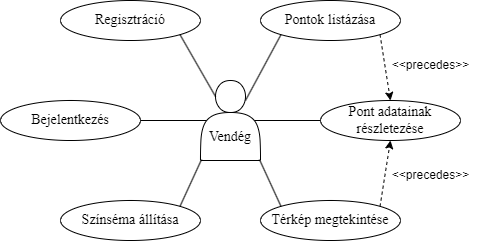
\includegraphics[width=0.75\textwidth]{usecase_guest}
	\caption{Felhasználói esetek vendégként}
	\label{fig:usecase_guest}
\end{figure}

\subsection{Felület általános leírása}

A weboldal látogatása során több felület is megjelenik, viszont ezek általánosan leírhatóak. Minden lap tetején egy navigációs sáv van, melynek segítségével több funkciót is gyorsan elérhetünk. A sáv bal oldalán a weboldal neve, illetve a "Térkép" felirat egyaránt a térképre, azaz a főoldalra irányít, a mellette szereplő "Lista" pedig a pontok listájához. A másik oldalon (jobbról balra) egy fizikai kapcsolót imitáló gomb, melynek segítségével válthatunk az előbb említett színsémák között, illetve amellett egy "Nincs bejelentkezve" feliratú listát lenyitva tudunk a regisztráció, illetve a bejelentkezés közül választani.\par
Ha a felhasználó nem egy széles képernyőn (pl. asztali számítógép vagy fektetett táblagép) látogatja meg az oldalt, akkor a sáv bár hasonlóan ott van, viszont a könnyebb használat érdekében a menüpontok egy, a jobb oldalon található \hspace{0.1cm}\boldmath\(\equiv\)\hspace{0.1cm} ikonra kattintva lehet ezeket elérni.

\begin{figure}[H]
	\centering
	\subcaptionbox{Nagy méretű kijelző}{
		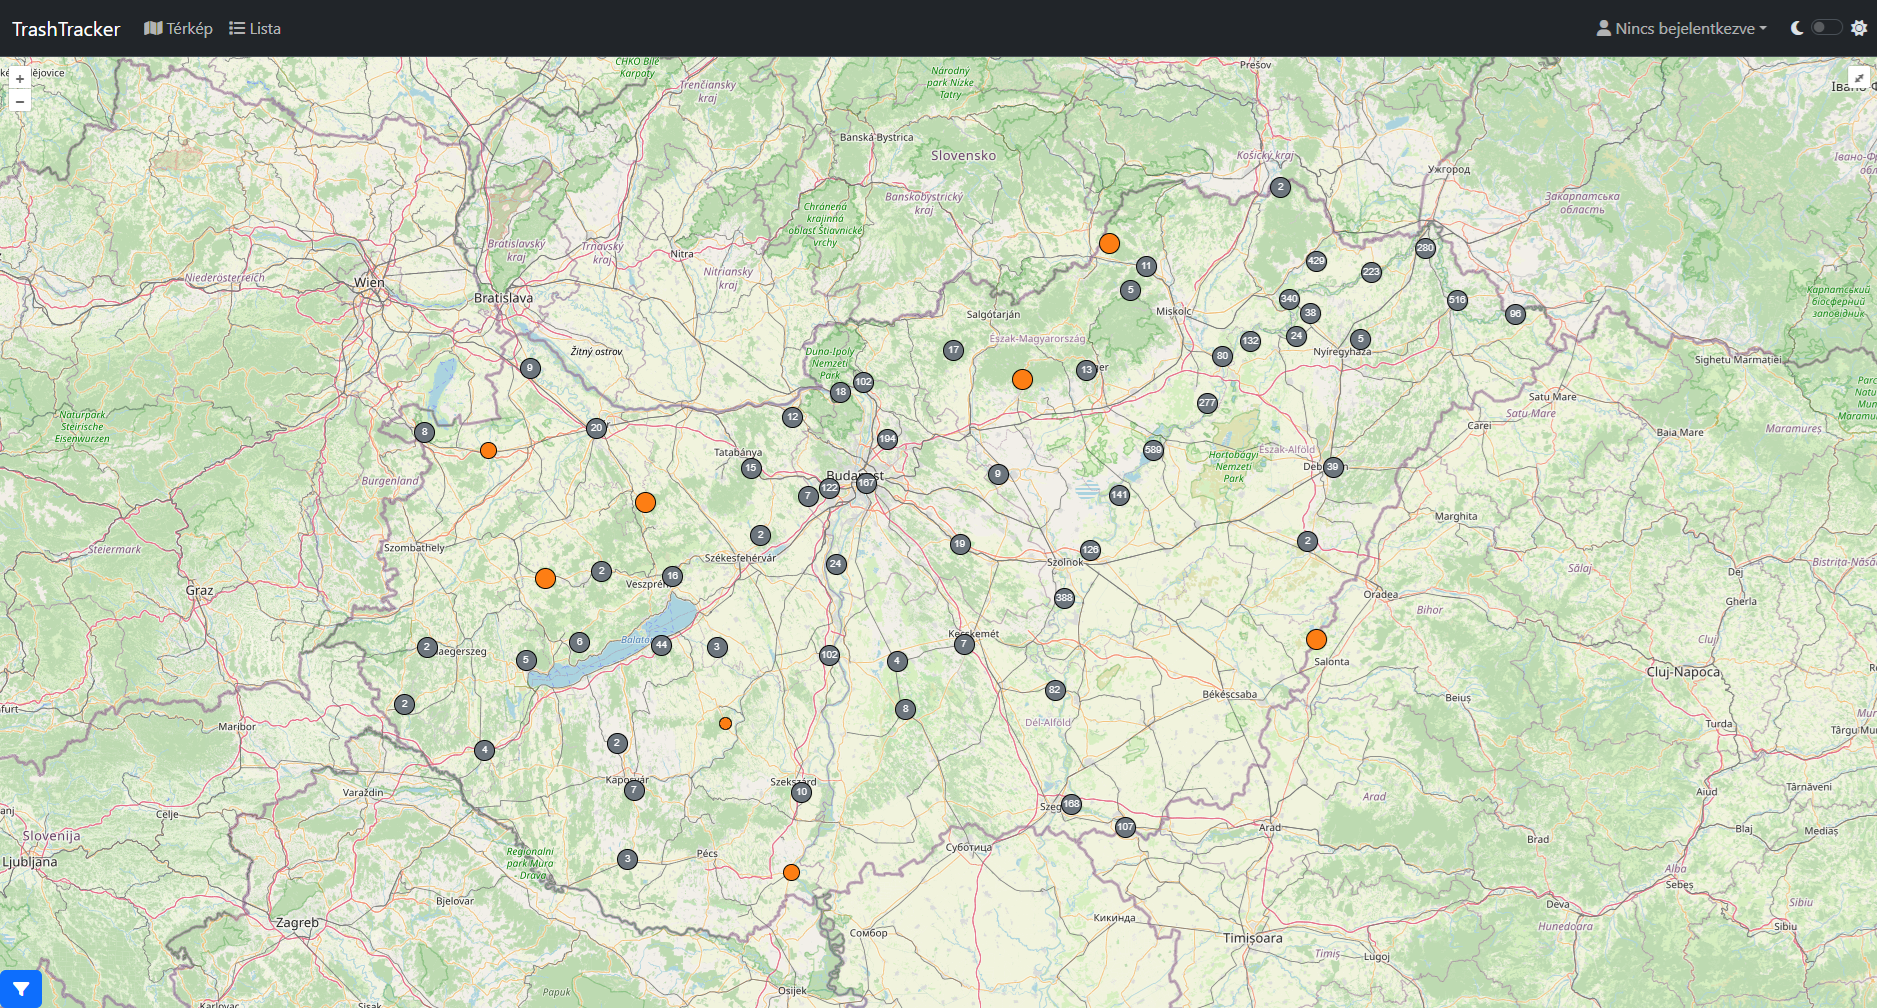
\includegraphics[width=0.45\linewidth]{map}}
	\hspace{5pt}
	\subcaptionbox{Kis méretű kijelző}{
		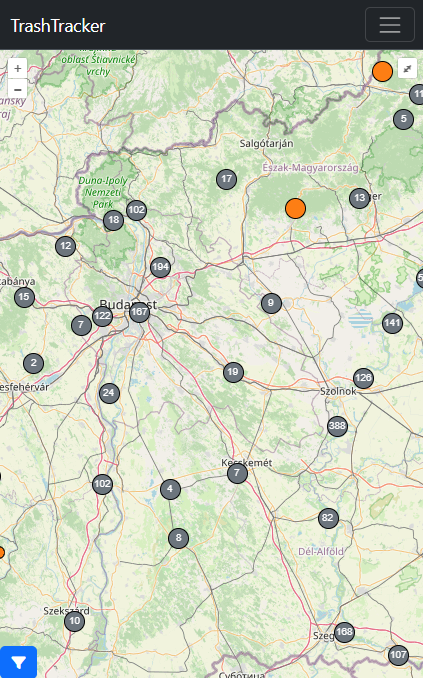
\includegraphics[width=0.2\linewidth]{map_phone}}
		\hspace{5pt}
	\subcaptionbox{Kis méretű kijelző (lenyitott navigációs sávval)}{
		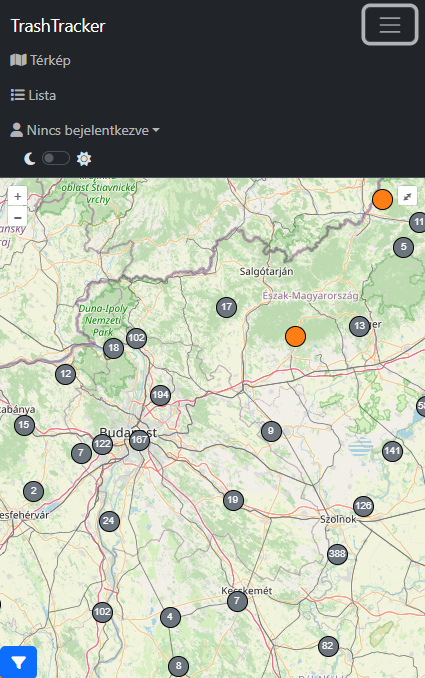
\includegraphics[width=0.2\linewidth]{map_phone_menu}}
	\caption{A felület kinézete a kezdőoldalon különböző méretű kijelzők esetén}
	\label{fig:map_guest}
\end{figure}

\subsection{Térkép (kezdőoldal)}

A navigációs sávon a weboldal nevére, illetve a "Térkép" feliratra kattintva azonnal a bejelentett pontok térképére navigálhatunk. Ennek kezelése a már jól ismert térképes alkalmazásokéhoz hasonló. A bal felső sarokban található \hspace{0.1cm}\boldmath\(+\)\hspace{0.1cm}, illetve \hspace{0.1cm}\boldmath\(-\)\hspace{0.1cm} ikonra kattintva nagyítani, illetve kicsinyíteni lehet, emellett egérrel a görgő görgetésével és érintőképernyőn két ujj összehúzásával/széttolásával is lehetőség van. A jobb felső sarokban a térképet teljes képernyős módba is lehet helyezni, melynek ismételt megnyomásával, vagy billentyűzeten az Esc gombbal ki lehet lépni. A bal alsó sarokban található a szűrés gomb, melynek segítségével különböző, a felhasználók által jelentett tulajdonságok szerint van lehetőség.

\subsubsection{Jelmagyarázat}

A térképen a pontok különböző mérettel és színnel jelennek meg, melyeknek céljuk a fontosabb információk lehetőség szerinti kiemelése.\\
A szemét mennyisége szerint a pont mérete lehet
\begin{compactitem}
	\item[\large\textbullet] kicsi (8 pixel), azaz "elfér egy zsákban",
	\item[\Large\textbullet] közepes (10 pixel), azaz "elfér egy talicskában" és
	\item[\LARGE\textbullet] nagy (12 pixel), azaz "autóra van szükség".
\end{compactitem}\newpage
A szemét első bejelentés óta levő állapota szerint a pont színe lehet
\begin{compactitem}
	\item[\textcolor{tt_green}{\Large\textbullet}] zöld, azaz "megtisztítva",
	\item[\textcolor{tt_yellow}{\Large\textbullet}] sárga, azaz "kevesebb",
	\item[\textcolor{tt_orange}{\Large\textbullet}] narancs, azaz "még mindig itt van" és
	\item[\textcolor{tt_red}{\Large\textbullet}] piros, azaz "több".
\end{compactitem}

\subsubsection{Szűrés}

A fentebb említett szűrés gombra kattintva a képernyő alján beúszik egy görgethető menü, amely a pontok tulajdonságai szerinti szűrést teszi lehetővé. A szemét mennyisége és állapota mellett annak típusa és hozzáférhetősége szerint is lehet válogatni. Ezeket a beúszó menün található, tulajdonságok szerint csoportosított "kapcsoló" gombokkal lehet elérni. Ha egy ilyen gomb kék színű, akkor igen, ha átlátszó, akkor pedig nem szeretnénk a térképen látni. Alapértelmezetten az összes ilyen gomb "igen" állapotban van. A gombok között szűrés esetén a logikai vagy művelete értelmezett, tehát ha bejelölésre kerül egy tulajdonság, viszont egy másik nem, akkor attól függetlenül a bejelöletlen attribútum még előfordulhat a megjelenített pontok között, feltéve, hogy legalább egy bejelölt jellemzővel rendelkezik. Ezt a menüt a jobb felső sarokban található \hspace{0.1cm}\boldmath\(\times\)\hspace{0.1cm} gombra nyomva lehet bezárni, a szűrőket megtartva, egy másik oldalra navigálásig vagy az oldal újratöltéséig.

\begin{figure}[H]
	\centering
	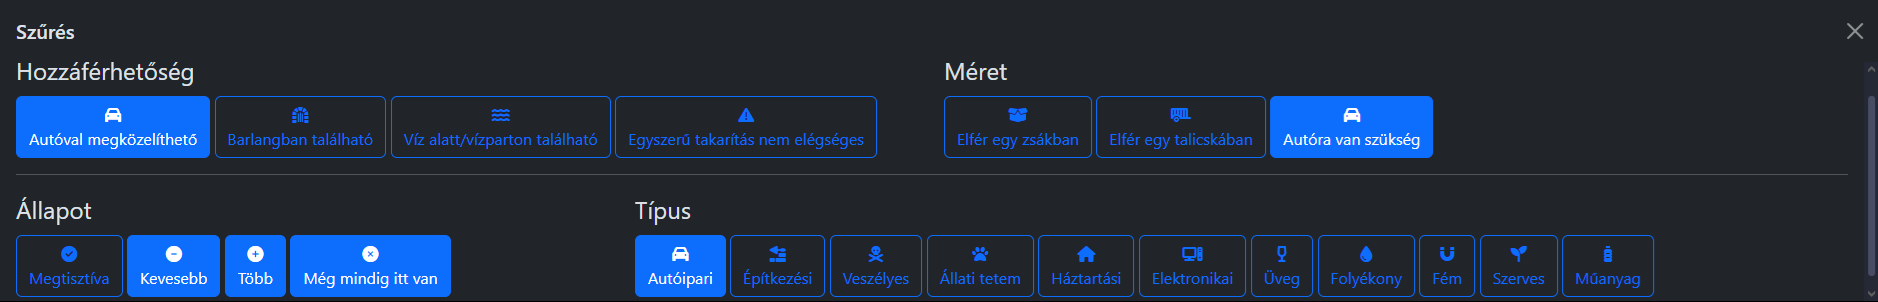
\includegraphics[width=1\textwidth]{map_filter}
	\caption{A kezdőoldal alján beúszó szűrési menü}
	\label{fig:map_filter}
\end{figure}

\subsubsection{Betekintés és részletek}

Egy pontra való kattintáskor afelett megjelenik egy modális "buborék", amely minimális információt és egy képet tartalmaz a hozzátartozó szemétről. Emellett a kis ablak alján található egy "Részletek" gomb, melyre kattintva elnavigálhatunk az azt részletező adatlapra.

\begin{figure}[H]
	\centering
	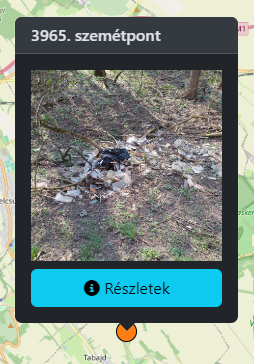
\includegraphics[width=0.225\textwidth]{map_popover}
	\caption{Példa egy felbukkanó buborékra egy ponton}
	\label{fig:map_popover}
\end{figure}

\subsection{Pont részletezése}

Ezt az oldalt az előző bekezdésben említett "Részletek" gombra kattintva, vagy a következő bekezdésben tárgyalt \faIcon{info-circle} ikonra kattintva lehet elérni. Itt az egyszerű tulajdonságok részletezésén túl megtalálható a pont pontos helyzete, illetve annak forrása (felhasználó esetén bejelentője). Előbbire kattintva a térképen levő helyére, utóbbira pedig annak forrására (TrashOut esetén az ottani adatlapjára, felhasználó esetén annak a profiljára) lehet navigálni.

\begin{figure}[H]
	\centering
	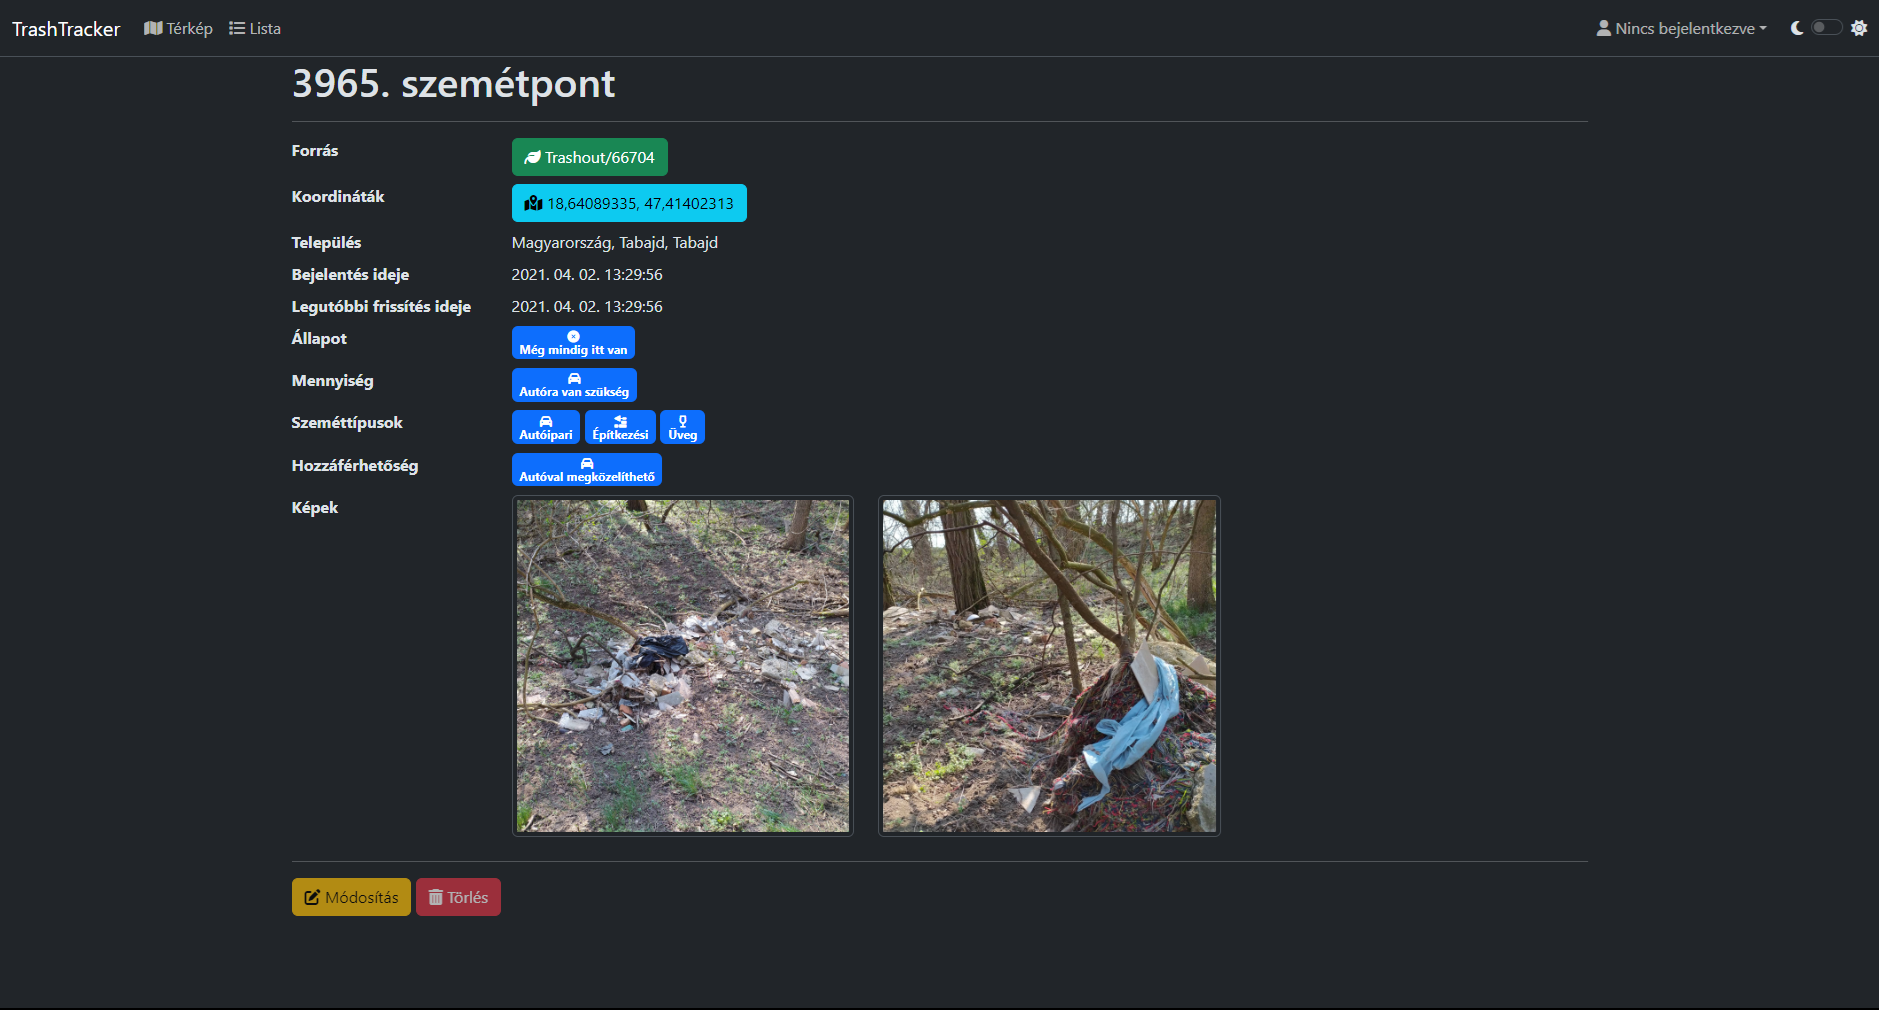
\includegraphics[width=0.7\textwidth]{trash_details}
	\caption{Példa egy szemétpontot részletező adatlapra}
	\label{fig:trash_details}
\end{figure}

\subsection{Listanézet}

A pontokat nem csak térképen, hanem listaként is megtekinthetjük. Ennek célja, hogy a bejelentés/frissítés dátuma szerint rendezve könnyedén fel lehessen fedezni a legrelevánsabb szemétlerakatokat. A lista minden sora egy-egy pontot, annak oszlopai pedig annak a fejlécben szereplő tulajdonságát tartalmazzák. Egy adott rekord részletezésére is lehetőség van, a jobb oldalon található \faIcon{info-circle} ikonra kattintva. Az oldal tetején lehetőség van alapvető szűrésekre is, opcionálisan belefoghatjuk a listába a már megtisztított pontokat, kereshetünk a bejelentő felhasználónevében, illetve az ahhoz tartozó megjegyzéseiben, illetve állíthatjuk az egy oldalon szereplő találatok maximális számát. Ha több találat van, mint ami az oldalon elfér, akkor a lista tetején, illetve alján található nyilakkal és számokkal könnyedén navigálhatunk azok között.

\begin{figure}[H]
	\centering
	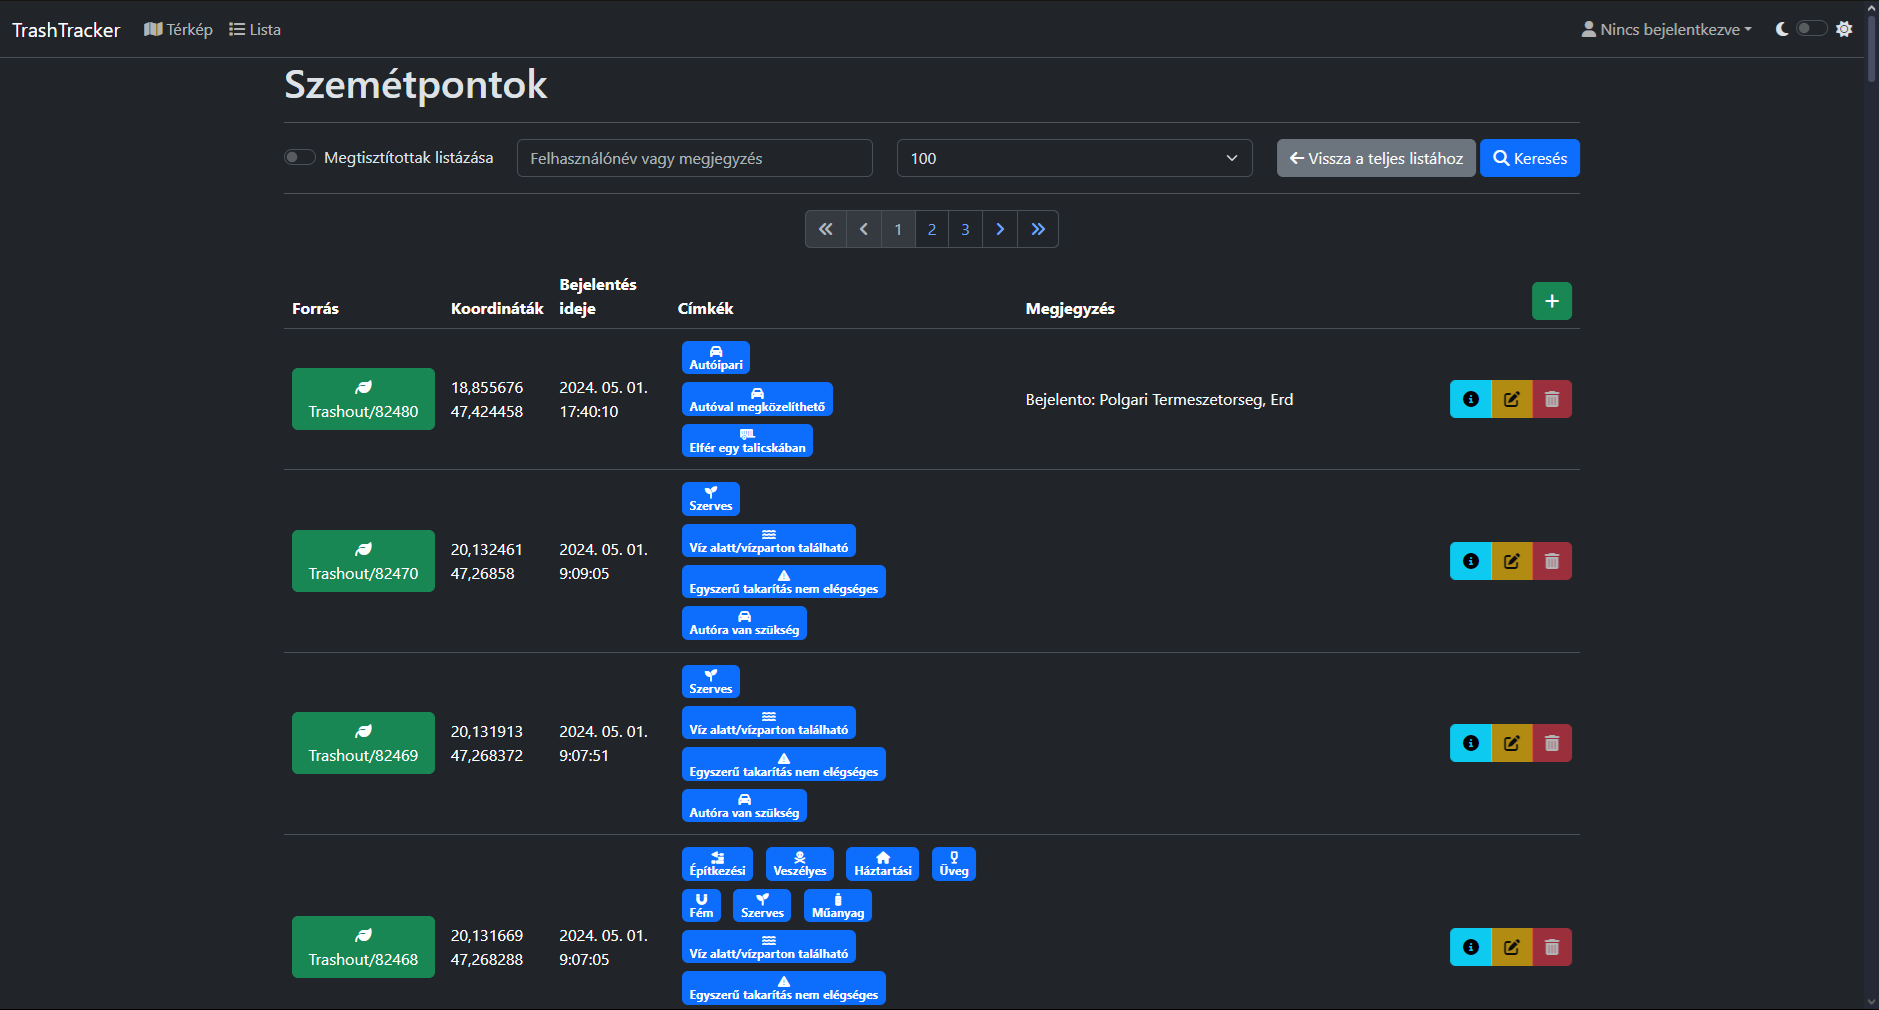
\includegraphics[width=0.7\textwidth]{trash_index}
	\caption{Szemétpontok listanézetének felülete}
	\label{fig:trash_index}
\end{figure}


\subsection{Színséma választása}

Minden oldal navigációs sávjának jobb szélén található egy kapcsoló mellyel könnyedén állítható az adott oldal színsémája, melynek bal- (\faIcon{moon}) állása sötét, illetve jobb oldali (\faIcon{sun}) állása világos módot jelent. Alapértelmezetten ez az előbbi állapotban van az energiatakarékosabb működés és a szemet jobban kímélő megjelenés miatt. Ez a beállítás szabadon állítható, mely megmarad minden aloldalon a böngészés idejére.

\begin{figure}[H]
	\centering
	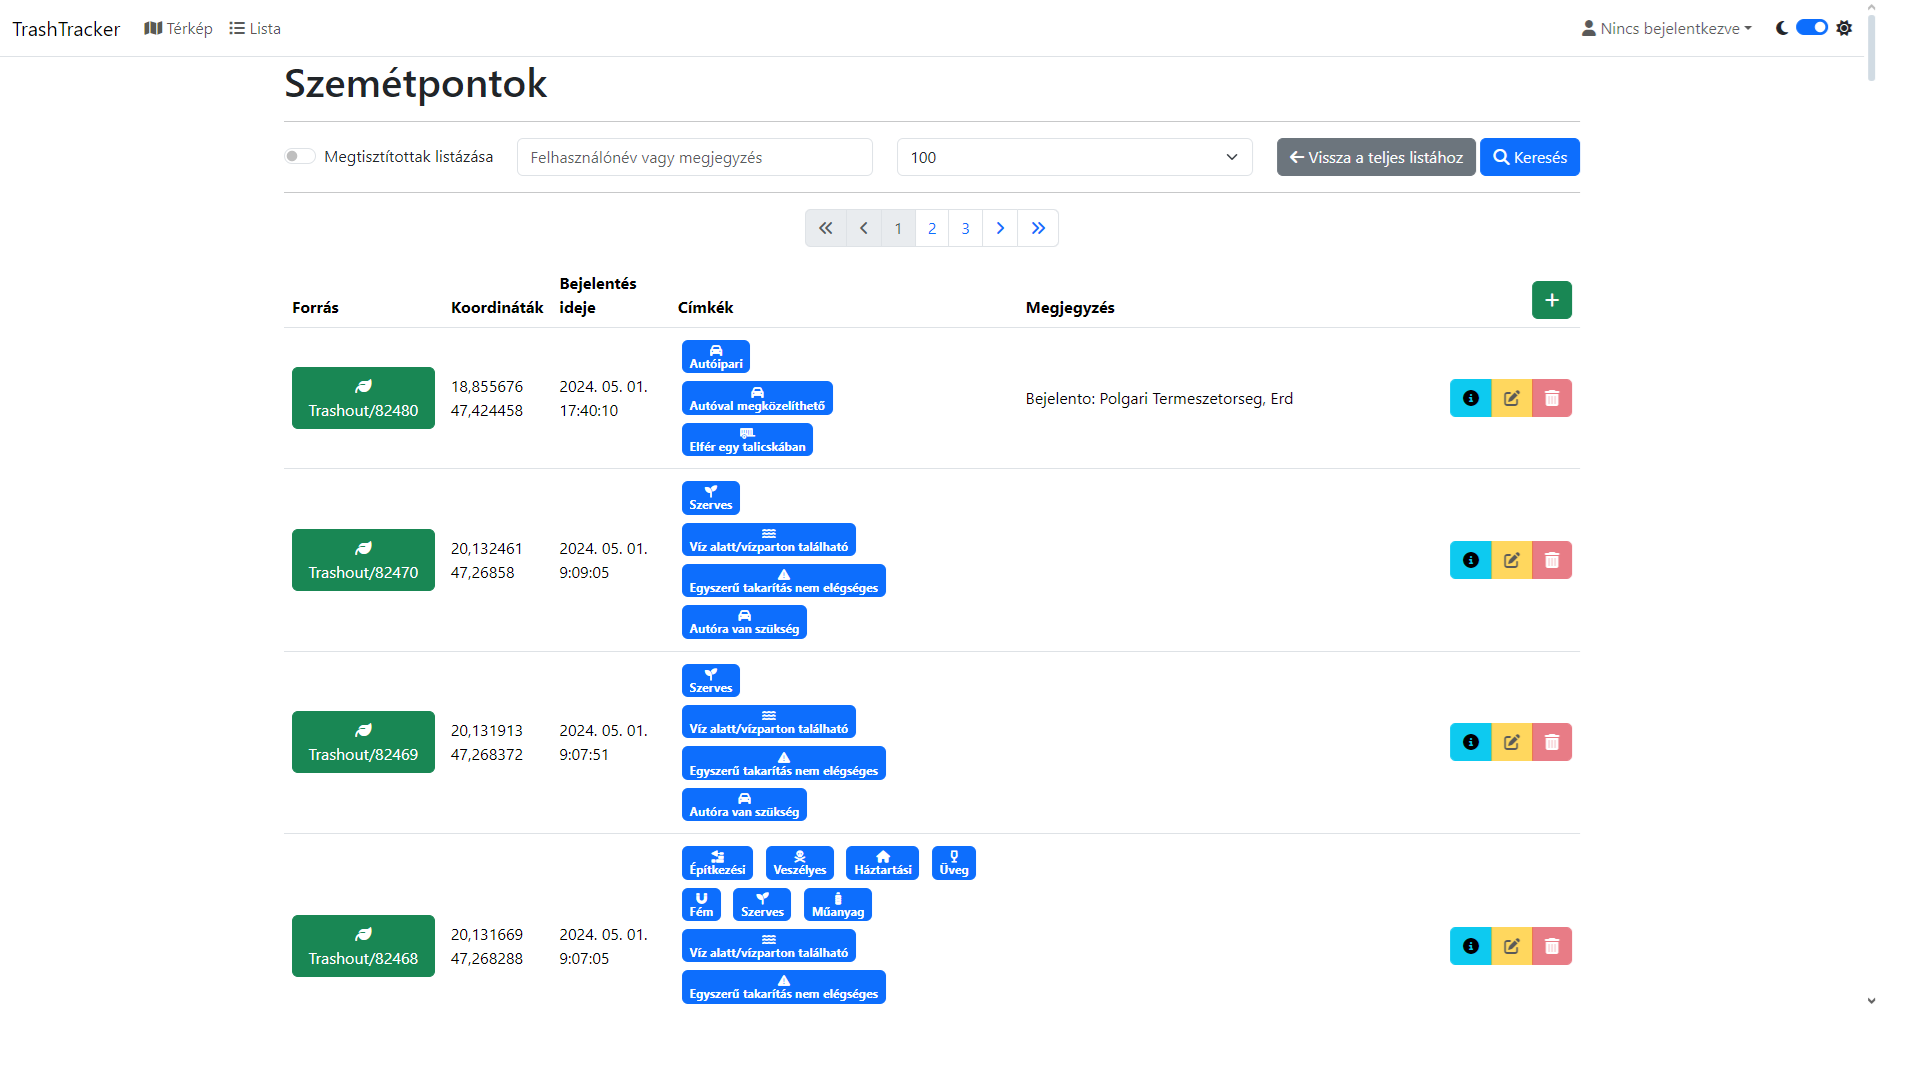
\includegraphics[width=0.7\textwidth]{trash_index_light}
	\caption{Szemétpontok listanézetének felülete világos módban}
	\label{fig:trash_index_light}
\end{figure}

\subsection{Regisztráció}

További funkciók használatáért (pontok bejelentése és frissítése) a felhasználónak egy felhasználói fiókra van szüksége, mely utóbbija ha nincs, akkor regisztrálnia kell hozzá. Ezt a navigációs sáv jobb oldalán található "Nincs bejelentkezve" feliratra kattintva lenyíló menüben szereplő "Regisztráció" menüpontra nyomva érheti el. Ha az előbbi helyett egy \faIcon{user} ikonnal társulva egy felhasználó neve szerepel, akkor az már be van jelentkezve, ezzel kapcsolatosan nincsen teendője.\par
A regisztrációs felületen egy űrlap található, ahol meg kell adni a kívánt felhasználónevet, e-mail címet (elérhetőségként), jelszavat, illetve opcionálisan egy profilképet. Az adatok kitöltése után az űrlap alján található "Regisztráció" gombra kattintva lehet beadni az adatokat, melyek ha megfelelnek a követelményeknek, akkor a felhasználó a főoldalon találja magát, az új fiókjával bejelentkezve.

\begin{figure}[H]
	\centering
	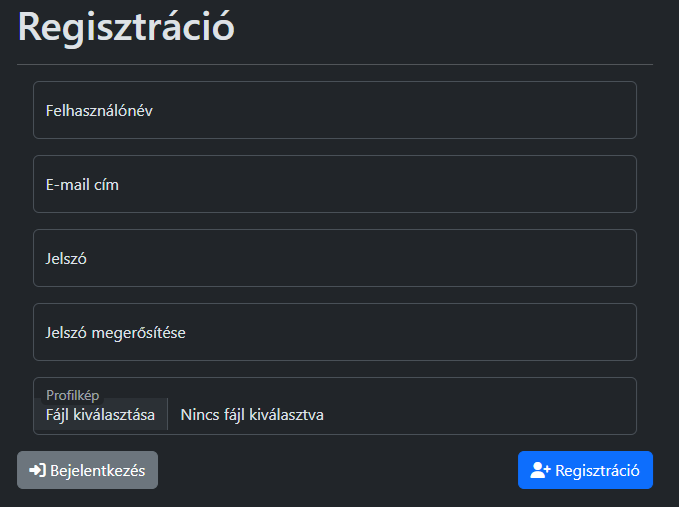
\includegraphics[width=0.7\textwidth]{register_form}
	\caption{A regisztrációs felület űrlapja}
	\label{fig:register_form}
\end{figure}

\subsubsection{Hibaüzenetek}

A regisztrációkor megadott adatok több követelménynek is meg kell hogy feleljenek, melyek "megsértésekor" hibaüzenetek jelenhetnek meg az űrlap kitöltése közben vagy után. Az első ilyen követelmény, hogy minden felhasználónévnek egyedinek kell lennie. Ezt az űrlap helyes kitöltése és elküldése után egy "\textcolor{red}{Ez a felhasználónév már foglalt!}" felirat jelzi.

\begin{figure}[H]
	\centering
	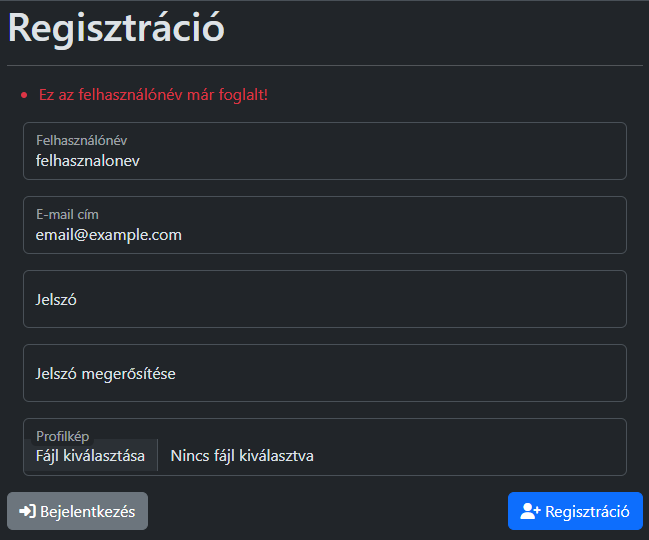
\includegraphics[width=0.7\textwidth]{register_form_duplicate_username}
	\caption{Már foglalt felhasználónév esetén megjelenő hibaüzenet}
	\label{fig:register_form_duplicate_username}
\end{figure}

Ha a megadott e-mail cím nem érvényes (azaz nem felel meg annak formai követelményeihez, pl. legyen benne "@" és egy "."), azt az űrlap kitöltése közben jelzi egy "\textcolor{red}{Érvénytelen e-mail cím!}" feliratú üzenet.

\begin{figure}[H]
	\centering
	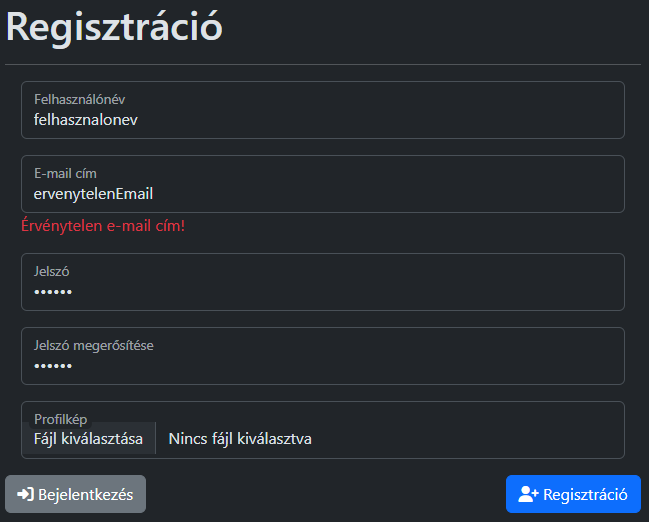
\includegraphics[width=0.7\textwidth]{register_form_invalid_email}
	\caption{Érvénytelen e-mail cím esetén megjelenő hibaüzenet}
	\label{fig:register_form_invalid_email}
\end{figure}

A legtöbb követelmény a jelszavakat érinti, itt több hibaüzenettel is találkozhat a felhasználó. Biztonsági okokból, egy jelszó 6-32 db karakterből kell álljon, melynek tartalmaznia kell legalább egy-egy kis- és nagybetűt, illetve számjegyet is. Ha ennek mégsem felelne meg a megadott jelszó, akkor azt az e-mail címhez hasonlóan egy "\textcolor{red}{A jelszó nem lehet rövidebb 6 és hosszabb 32 karakternél!}" vagy "\textcolor{red}{Jelszónak tartalmaznia kell legalább egy kis- és nagybetűt illetve számjegyet!}" üzenet jelenik meg, annak függvényében, hogy melyik pontján nem megy át az ellenőrzésen (tehát ha túl rövid a jelszó és pl. nem tartalmaz nagybetűt, akkor csak az előbbi jelenik meg, az utóbbi csak ha a hossz javítása után sem felel meg). Emellett a jelszó megerősítésére is szükség van, azaz meg kell adni a beírt jelszót egy második alkalommal is. Ha ezek nem egyeznének meg, azt is egy hibaüzenet jelzi a felhasználó számára.

\begin{figure}[H]
	\centering
	\subcaptionbox{Nem megfelelő hosszú jelszó hibaüzenete}{
		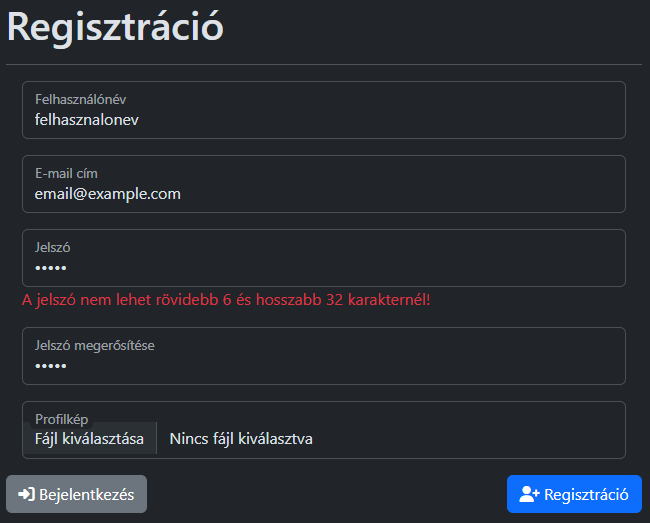
\includegraphics[width=0.3\linewidth]{register_form_invalid_password_length}}
	\hspace{5pt}
	\subcaptionbox{Nem megfelelő karaktereket tartalmazó jelszó hibaüzenete}{
		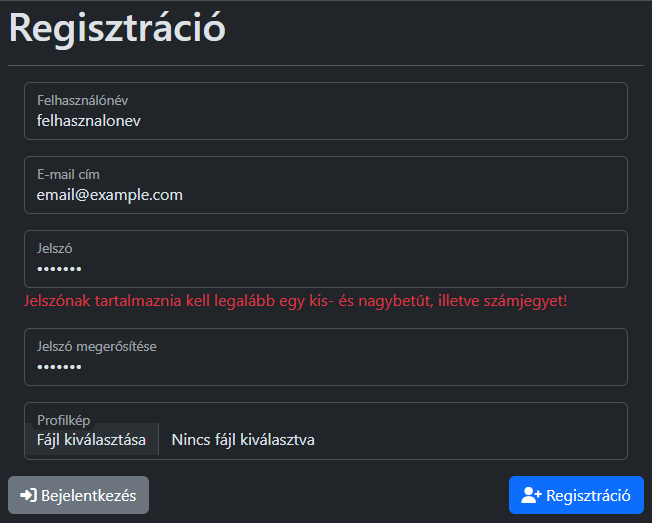
\includegraphics[width=0.3\linewidth]{register_form_invalid_password_characters}}
	\hspace{5pt}
	\subcaptionbox{Nem azonos jelszavak hibaüzenete}{
		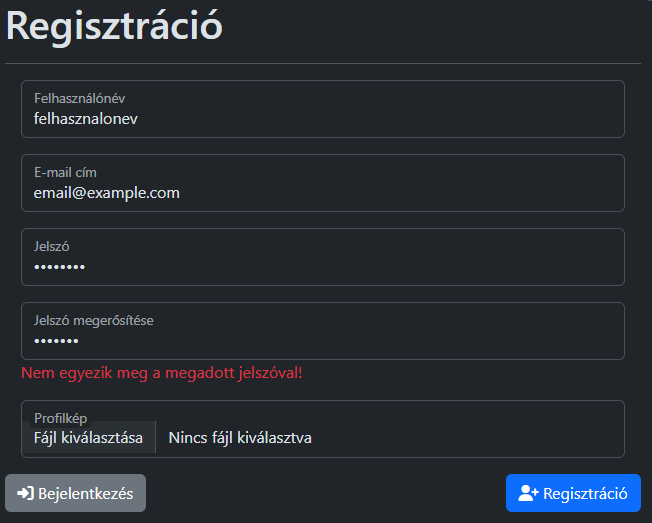
\includegraphics[width=0.3\linewidth]{register_form_invalid_password_repeat}}
	\caption{Érvénytelen jelszó esetén megjelenő hibaüzenetek}
	\label{fig:register_form_invalid_password}
\end{figure}

\subsection{Bejelentkezés}

Ha a felhasználónak már van saját fiókja, akkor ismételt regisztráció helyett beléphet abba, az előző bekezdésben tárgyaltak szerint a "Bejelentkezés" gombra kattintva. Az űrlap hasonló, viszont itt elég csak a felhasználónév (vagy e-mail cím tetszőlegesen), illetve a hozzátartozó jelszó egyszeri megadására. Ha az adatok egyeznek a regisztrációkor megadottakkal, akkor az űrlap alján található "Bejelentkezés" gombra kattintva a felhasználó a főoldalra lesz átirányítva, a felhasználói fiókjába bejelentkezve. Ellenben, ha nem jár sikerrel, akkor üzenetek tájékoztatják a klienst erről. Ha többszöri próbálkozásra sem jár sikerrel, akkor lehetősége van bejelentkezés helyett újabb felhasználó regisztrálására, vagy egy adminisztrátort megkérve bejelentkezési adatainak megváltoztatására is.

\begin{figure}[H]
	\centering
	
\includegraphics[width=0.7\textwidth]{login_form}
	\caption{A bejelentkezéses felület űrlapja}
	\label{fig:login_form}
\end{figure}

\subsubsection{Hibaüzenetek}

Sikertelen bejelentkezés esetén, azaz nem megfelelő felhasználónév (vagy e-mail cím) és jelszó páros megadásakor biztonsági okok miatt csak egy, a regisztráláskor látottaknál általánosabb "\textcolor{red}{Sikertelen bejelentkezés!}" felirat szerepel.

\begin{figure}[H]
	\centering
	
\includegraphics[width=0.7\textwidth]{login_form_error}
	\caption{A bejelentkezéses felület űrlapján szereplő hibaüzenet}
	\label{fig:login_form_error}
\end{figure}

\section{Funkciók felhasználóként}

Sikeres bejelentkezést (vagy regisztrációt) követően a felhasználó vendég helyett bejelentkezett felhasználónak (vagy fióktípusának megfelelőnek) számít. Ezzel további funkciók válnak elérhetővé, mint például a szemétpontok bejelentése és frissítése, illetve a saját felhasználói fiók profiljának szerkesztése.

\begin{figure}[H]
	\centering
	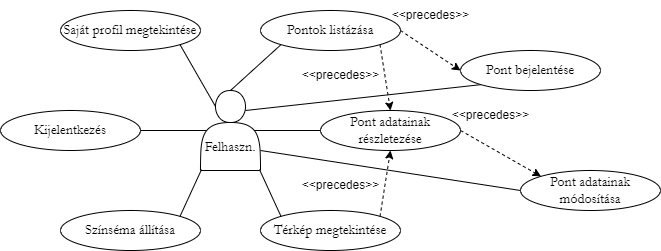
\includegraphics[width=0.7\textwidth]{usecase_user}
	\caption{Felhasználói esetek (bejelentkezett) felhasználóként}
	\label{fig:usecase_user}
\end{figure}

\subsection{Pont bejelentése}

Új pont bejelentésére a listanézet tetején található \faIcon{plus} ikonra kattintva van lehetőség, mely elnavigál annak az űrlapjára. Ezen az űrlapon meg kell adni a szemét pontos helyzetét koordinátákként, amely megadásának segítségül szolgál a szöveges mezőjük melletti "Jelenlegi hely meghatározása", mely megnyomásával a böngésző meghatározza a bejelentőnek a lehető legpontosabb koordinátáit. A méret jellemzése mellett ajánlott a szemét típusát és hozzáférhetőségét is megadni, melynek kezelése hasonló a térképen való szűrés gombjaihoz. Az utolsó, többsoros szöveges mezőben megjegyzést lehet írni, mely segíti a listanézetben való keresését a pontnak.

\subsubsection{Hibaüzenetek}

\subsection{Pont módosítása}

Egy már meglévő pont adatainak módosítására az azt részletező adatlap alján található "Módosítás", vagy a listanézet egyes soraiban található \faIcon{edit} ikonra kattintva érhető el. Az ezen az oldalon található űrlap hasonló, a pont létrehozáskor használtéhoz, a szemét állapotának lenyíló menüjét leszámítva, melynek megadása létrehozáskor még értelmetlen lenne.

\subsubsection{Hibaüzenetek}

\section{Felsorolások}

Etiam vel odio ante. Etiam pulvinar nibh quis massa auctor congue. Pellentesque quis odio vitae sapien molestie vestibulum sit amet et quam. Pellentesque vel dui eget enim hendrerit finibus at sit amet libero. Quisque sollicitudin ultrices enim, nec porta magna imperdiet vitae. Cras condimentum nunc dui, eget molestie nunc accumsan vel.

\begin{itemize}
	\item Fusce in aliquet neque, in pretium sem.
	\item Donec tincidunt tellus id lectus pretium fringilla.
	\item Nunc faucibus, erat pretium tempus tempor, tortor mi fringilla neque, ac congue ex dui vitae mauris.
\end{itemize}

Donec dapibus sodales ante, at scelerisque nunc laoreet sit amet. Mauris porttitor tincidunt neque, vel ullamcorper neque pulvinar et. Integer eu lorem euismod, faucibus lectus sed, accumsan felis. Nunc ornare mi at augue vulputate, eu venenatis magna mollis. Nunc sed posuere dui, et varius nulla. Sed mollis nibh augue, eget scelerisque eros ornare nec.

\begin{enumerate}
	\item\label{step:first} Donec pretium et quam a cursus. Ut sollicitudin tempus urna et mollis.
	\item Aliquam et aliquam turpis, sed fermentum mauris. Nulla eget ex diam.
	\item Donec eget tellus pharetra, semper neque eget, rutrum diam \ref{step:first}.~lépés.
\end{enumerate}

Praesent porta, metus eget eleifend consequat, eros ligula eleifend ex, a pellentesque mi est vitae urna. Vivamus turpis nunc, iaculis non leo eget, mattis vulputate tellus. Maecenas rutrum eros sem, pharetra interdum nulla porttitor sit amet. In vitae viverra ante. Maecenas sit amet placerat orci, sed tincidunt velit. Vivamus mattis, enim vel suscipit elementum, quam odio venenatis elit\footnote{Phasellus faucibus varius purus, nec tristique enim porta vitae.}, et mollis nulla nunc a risus. Praesent purus magna, tristique sed lacus sit amet, convallis malesuada magna. 

\begin{description}
	\item[Vestibulum venenatis] malesuada enim, ac auctor erat vestibulum et. Phasellus id purus a leo suscipit accumsan.
	\item[Orci varius natoque] penatibus et magnis dis parturient montes, nascetur ridiculus mus. Nullam interdum rhoncus nisl, vel pharetra arcu euismod sagittis. Vestibulum ac turpis auctor, viverra turpis at, tempus tellus.
	\item[Morbi dignissim] erat ut rutrum aliquet. Nulla eu rutrum urna. Integer non urna at mauris scelerisque rutrum sed non turpis.
\end{description}

\subsection{Szoros térközű felsorolások}

Phasellus ultricies, sapien sit amet ultricies placerat, velit purus viverra ligula, id consequat ipsum odio imperdiet enim:
\begin{compactenum}
	\item Maecenas eget lobortis leo.
	\item Donec eget libero enim.
	\item In eu eros a eros lacinia maximus ullamcorper eget augue.
\end{compactenum}

\bigskip

In quis turpis metus. Proin maximus nibh et massa eleifend, a feugiat augue porta. Sed eget est purus. Duis in placerat leo. Donec pharetra eros nec enim convallis:
\begin{compactitem}
	\item Pellentesque odio lacus.
	\item Maximus ut nisl auctor.
	\item Sagittis vulputate lorem.
\end{compactitem}

\bigskip

Vestibulum ante ipsum primis in faucibus orci luctus et ultrices posuere cubilia Curae; Sed lorem libero, dignissim vitae gravida a, ornare vitae est.
\begin{compactdesc}
	\item[Cras maximus] massa commodo pellentesque viverra.
	\item[Morbi sit] amet ante risus. Aliquam nec sollicitudin mauris
	\item[Ut aliquam rhoncus sapien] luctus viverra arcu iaculis posuere
\end{compactdesc}


\section{Képek, ábrák}

Aliquam vehicula luctus mi a pretium. Nulla quam neque, maximus nec velit in, aliquam mollis tortor. Aliquam erat volutpat. Curabitur vitae laoreet turpis. Integer id diam ligula. Nulla sodales purus id mi consequat, eu venenatis odio pharetra. Cras a arcu quam. Suspendisse augue risus, pulvinar a turpis et, commodo aliquet turpis. Nulla aliquam scelerisque mi eget pharetra. Mauris sed posuere elit, ac lobortis metus. Proin lacinia sit amet diam sed auctor. Nam viverra orci id sapien sollicitudin, a aliquam lacus suscipit, \ref{fig:example-1}.~ábra:

\begin{figure}[H]
	\centering
	
\includegraphics[width=0.6\textwidth,height=100px]{elte_cimer_szines}
	\caption{Quisque ac tincidunt leo}
	\label{fig:example-1}
\end{figure}

\subsection{Képek szegélyezése}

Ut aliquet nec neque eget fermentum. Cras volutpat tellus sed placerat elementum. Quisque neque dui, consectetur nec finibus eget, blandit id purus. Nam eget ipsum non nunc placerat interdum.

\begin{figure}[H]
	\centering
	
\includegraphics[width=0.6\textwidth,height=100px,frame]{elte_cimer_szines}
	\caption{Quisque ac tincidunt leo}
\end{figure}

\subsection{Képek csoportosítása}

In non ipsum fermentum urna feugiat rutrum a at odio. Pellentesque habitant morbi tristique senectus et netus et malesuada fames ac turpis egestas. Nulla tincidunt mattis nisl id suscipit. Sed bibendum ac felis sed volutpat. Nam pharetra nisi nec facilisis faucibus. Aenean tristique nec libero non commodo. Nulla egestas laoreet tempus. Nunc eu aliquet nulla, quis vehicula dui. Proin ac risus sodales, gravida nisi vitae, efficitur neque, \ref{fig:example-2}.~ábra:

\begin{figure}[H]
	\centering
	\subcaptionbox{Vestibulum quis mattis urna}{
		
\includegraphics[width=0.45\linewidth]{elte_cimer_szines}}
	\hspace{5pt}
	\subcaptionbox{Donec hendrerit quis dui sit amet venenatis}{
		
\includegraphics[width=0.45\linewidth]{elte_cimer_szines}}
	\caption{Aenean porttitor mi volutpat massa gravida}
	\label{fig:example-2}
\end{figure}

Nam et nunc eget elit tincidunt sollicitudin. Quisque ligula ipsum, tempor vitae tortor ut, commodo rhoncus diam. Pellentesque habitant morbi tristique senectus et netus et malesuada fames ac turpis egestas. Phasellus vehicula quam dui, eu convallis metus porta ac.


\section{Táblázatok}

Nam magna ex, euismod nec interdum sed, sagittis nec leo. Nam blandit massa bibendum mattis tristique. Phasellus tortor ligula, sodales a consectetur vitae, placerat vitae dolor. Aenean consequat in quam ac mollis. 

\begin{table}[H]
	\centering
	\begin{tabular}{ | m{0.25\textwidth} | m{0.65\textwidth} | }
		\hline
		\textbf{Phasellus tortor} & \textbf{Aenean consequat} \\
		\hline \hline
		\emph{Sed malesuada} & Aliquam aliquam velit in convallis ultrices. \\
		\hline
		\emph{Purus sagittis} &  Quisque lobortis eros vitae urna lacinia euismod. \\
		\hline
		\emph{Pellentesque} & Curabitur ac lacus pellentesque, eleifend sem ut, placerat enim. Ut auctor tempor odio ut dapibus. \\
		\hline
	\end{tabular}
	\caption{Maecenas tincidunt non justo quis accumsan}
	\label{tab:example-1}
\end{table}

\subsection{Sorok és oszlopok egyesítése}

Mauris a dapibus lectus. Vestibulum commodo nibh ante, ut maximus magna eleifend vel. Integer vehicula elit non lacus lacinia, vitae porttitor dolor ultrices. Vivamus gravida faucibus efficitur. Ut non erat quis arcu vehicula lacinia. Nulla felis mauris, laoreet sed malesuada in, euismod et lacus. Aenean at finibus ipsum. Pellentesque dignissim elit sit amet lacus congue vulputate.

\begin{table}[htb]
	\centering
	\begin{tabular}{ | c | r | r | r | r | r | r | }
		\hline
		\multirow{2}{*}{\textbf{Quisque}} & \multicolumn{2}{ c | }{\textbf{Suspendisse}} & \multicolumn{2}{ c | }{\textbf{Aliquam}} & \multicolumn{2}{ c | }{\textbf{Vivamus}} \\
		\cline{2-7}
		& Proin & Nunc & Proin & Nunc & Proin & Nunc \\
		\hline \hline		
		Leo & 2,80 MB & 100\% & 232 KB & 8,09\% & 248 KB & 8,64\% \\
		\hline
		Vel & 9,60 MB & 100\% & 564 KB & 5,74\% & 292 KB & 2,97\% \\
		\hline
		Auge & 78,2 MB & 100\% & 52,3 MB & 66,88\% & 3,22 MB & 4,12\% \\
		\hline 
	\end{tabular}
	\caption[Rövid cím a táblázatjegyzékbe]{Vivamus ac arcu fringilla, fermentum neque sed, interdum erat. Mauris bibendum mauris vitae enim mollis, et eleifend turpis aliquet.}
	\label{tab:example-2}
\end{table}

\subsection{Több oldalra átnyúló táblázatok}

Nunc porta placerat leo, sit amet porttitor dui porta molestie. Aliquam at fermentum mi. Maecenas vitae lorem at leo tincidunt volutpat at nec tortor. Vivamus semper lacus eu diam laoreet congue. Vivamus in ipsum risus. Nulla ullamcorper finibus mauris non aliquet. Vivamus elementum rhoncus ex ut porttitor.

\begin{center}
	\begin{longtable}{ | p{0.3\textwidth} | p{0.7\textwidth} | }
		
		\hline
		\multicolumn{2}{|c|}{\textbf{Praesent aliquam mauris enim}}
		\\ \hline
		
		\emph{Suspendisse potenti} & \emph{Lorem ipsum dolor sit amet}
		\\ \hline \hline
		\endfirsthead % első oldal fejléce
		
		\hline
		\emph{Suspendisse potenti} & \emph{Lorem ipsum dolor sit amet}
		\\ \hline \hline
		\endhead % többi oldal fejléce
		
		\hline
		\endfoot % többi oldal lábléce
		
		\endlastfoot % utolsó oldal lábléce
		
		\emph{Praesent}
		& Nulla ultrices et libero sit amet fringilla. Nunc scelerisque ante tempus sapien placerat convallis.
		\\ \hline
		
		\emph{Luctus}
		& Integer hendrerit erat massa, non hendrerit risus convallis at. Curabitur ultrices, justo in imperdiet condimentum, neque tortor luctus enim, luctus posuere massa erat vitae nibh.
		\\ \hline
		
		\emph{Egestas}
		& Duis fermentum feugiat augue in blandit. Mauris a tempor felis. Pellentesque ultricies tristique dignissim. Pellentesque aliquam semper tristique. Nam nec egestas dolor. Vestibulum id elit quis enim fringilla tempor eu a mauris. Aliquam vitae lacus tellus. Phasellus mauris lectus, aliquam id leo eget, auctor dapibus magna. Fusce lacinia felis ac elit luctus luctus.
		\\ \hline
		
		\emph{Dignissim}
		& Praesent aliquam mauris enim, vestibulum posuere massa facilisis in. Suspendisse potenti. Nam quam purus, rutrum eu augue ut, varius vehicula tellus. Fusce dui diam, aliquet sit amet eros at, sollicitudin facilisis quam. Phasellus tempor metus vel augue gravida pretium. Proin aliquam aliquam blandit. Nulla id tempus mi. Fusce in aliquam tortor.
		\\ \hline
		
		\emph{Pellentesque}
		& Donec felis nibh, imperdiet a arcu non, vehicula gravida nibh. Quisque interdum sapien eu massa commodo, ac elementum felis faucibus.
		\\ \hline
		
		\emph{Molestie}
		& Cras ullamcorper tellus et auctor ultricies. Maecenas tincidunt euismod lectus nec venenatis. Suspendisse potenti. Pellentesque pretium nunc ut euismod cursus. Nam venenatis condimentum quam. Curabitur suscipit efficitur aliquet. Interdum et malesuada fames ac ante ipsum primis in faucibus.
		\\ \hline
		
		\emph{Vivamus semper}
		& In purus purus, faucibus eu libero vulputate, tristique sodales nunc. Nulla ut gravida dolor. Fusce vel pellentesque mi, vel efficitur eros. Nunc vitae elit tellus. Sed vestibulum auctor consequat. 
		\\ \hline
		
		\emph{Condimentum}
		& Nulla scelerisque, leo et facilisis pretium, risus enim cursus turpis, eu suscipit ipsum ipsum in mauris. Praesent eget pulvinar ipsum, suscipit interdum nunc. Nam varius massa ut justo ullamcorper sollicitudin. Vivamus facilisis suscipit neque, eu fermentum risus. Ut at mi mauris.
		\\ \hline
		
		\caption{Praesent ullamcorper consequat tellus ut eleifend}
		\label{tab:example-3}		
	\end{longtable}
\end{center}